\documentclass[conference]{IEEEtran}
\usepackage{graphicx}
\usepackage{float}
\usepackage{cite}
\begin{document}
\title{ A Survey Paper on Hybrid Recommender Systems}
\author{\IEEEauthorblockN{Chandramani Adil}\IEEEauthorblockN{Computer Science and Engineering\\
Malaviya National Institute of Technology, Jaipur\\
}}
\maketitle
\begin{abstract}
\em
Recommender System is an Information filtering system that is used to predict the rating or preference a user would give to an item.In this Survey we are going to discuss about the various techniques like content-based, collaborative filtering etc. what are the issue they face and how the recommendations were improved by the hybrid recommender systems.
\end{abstract}

\section{INTRODUCTION}
In this modern era of online shopping a recommendation system 
has become an essential part of it as it helps the users to select the desired item without much hassles. A recommendation system applies various techniques like Content Filtering, Collaborative filtering to generate recommdneation for the active users.\cite{paper1}.
 
  The rest of the paper is organized as follows. Section II discusses about previous work done in the recommendation systems . This is followed by problems faced by classical approach of recommendation systems in Section III. Section IV describes the Hybrid Recommendation System types. Section V talks about the approaches used in Hybrid Recommendation Systems. At last, Section VI draws some important conclusions.

\section{Previous Work}
	Recommender system emerged as an independent research area in the mid 1990’s when researchers started focusing on recommendation problem that explicitly depends on the rating method.\\
	Specifically, recommender systems have (i) background data, the information that the
system has before the recommendation process begins, (ii) input data, the information that user must communicate to
the system in order to generate a recommendation, and (iii) an algorithm that combines background and input data to
arrive at its suggestions. On this basis, we can distinguish five different recommendation techniques as shown in
Table I. Assume that I is the set of items over which recommendations might be made, U is the set of users whose
preferences are known, u is the user for whom recommendations need to be generated, and i is some item for which
we would like to predict u’s preference.\cite{paper1}
\subsection{Collaborative Filtering}
	Collaborative filtering, also referred to as social filtering, filters information by using the recommendations of other people. It is based on the idea that people who agreed in their evaluation of certain items in the past are likely to agree again in the future.
	\begin{figure}[h]
  \caption{Example of Collaborative Filtering}
  \centering
    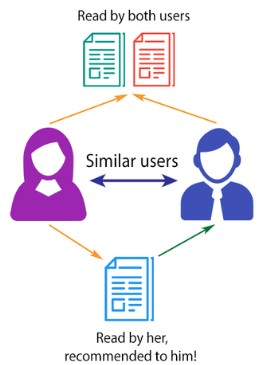
\includegraphics[width=0.3\textwidth]{collab}
\end{figure}

	Advantages	
	\begin{itemize}
	\item Easy implementation
	\item Addition of new data is easy
	\end{itemize}
	Disadvantages	
	\begin{itemize}
	\item Cold Start Problem 
	\item Scalability
	\item Scarsity
	\end{itemize}
	
\subsection{Content Based}
	Content-based filtering, also referred to as cognitive filtering, recommends items based on a comparison between the content of the items and a user profile. The content of each item is represented as a set of descriptors or terms, typically the words that occur in a document. The user profile is represented with the same terms and built up by analyzing the content of items which have been seen by the user.\\
	\begin{figure}[h]
  \caption{Example of Content-Based filtering.}
  \centering
    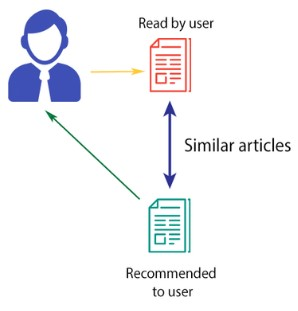
\includegraphics[width=0.3\textwidth]{content}
\end{figure}

	Advantages	
	\begin{itemize}
	\item Provides transparency to the active user.
	\item good at recommending items that are not yet rated.
	\end{itemize}
	Disadvantages	
	\begin{itemize}
	\item Difficult to generate characteristics of the item. 
	\item Over-Specialization
	\item Difficult to get feedback from the users.
	\end{itemize}	
	
	\begin{table}[h]
	
\begin{tabular}{|p{1.5cm}|p{1.5cm}|p{2cm}|p{2cm}|}
\hline
\textbf{technique} & \textbf{background} & \textbf{input} & \textbf{output} \\ \hline
Collaborative & Ratings from Users of items in Items & Ratings from Users & Identify users in Users similar \\ \hline
Content-Based & Features of items in Items & User's rating of items & generate a classifier that fits User's rating behaviour \\ \hline
Demographic & Demographic information about users & Demographic information about user & Identify all the users that are demographically similar to the User \\ \hline
Utility-Based & Features of items in Items & Utility function over items & Apply the function to the items and determines Items rank \\ \hline
Knowledge Based & Features of item in Items & A description of Users & Infer a match between Item's and User's need \\ \hline
\end{tabular}
\caption{Recommendation Techniques}
\label{Table1}
\end{table}
\subsection{Other Approaches}

	Other approaches include Demographic based, Utility based and Knowledge based.
	

\section{Problems}

	Issues related with above algorithms are:
		\begin{enumerate}
		\item Cold-Start\\
				It's difficult to provide recommendation to new users/item because we don't have any data related to those available with us.
		\item Scalability\\
				After a certain time when number of users and item increase, then the system needs more resources to give proper recommendation.
		\item Sparsity\\
				It's the lack/unavailability of required information to give proper recommendation.	
		\item Privacy\\
				It's a major issue in context to demographic recommender system, where system needs appropriate information to predict correctly.
		\item Over-Specialization\\
				This is a common problem where a system must suggest diverse items which content-based system lacks.
		\item Freshness(Predictability)\cite{paper2}\\
				Even if the items recommended to the user are diverse, it might be familiar to the user. 
		\end{enumerate}
	
\section{Hybrid Filtering}

	\subsection{Weighted}
		Scores/votes of several recommendation techniques are combined together to produce a single recommendation.
	\subsection{Switching}
		System switches between multiple recommendation techniques depending on the current situation. 
	\subsection{Mixed}
		Recommendation from several different recommenders are presented at the same time.
	\subsection{Feature Combination}
		Features from the different recommendation data sources are mixed together to form a single recommendation engine.
	\subsection{Cascade}
		One recommendation system refines the output given by another recommendation system.
	\subsection{Feature Augmentation}
		Output from one recommendation engine is used as an input feature to another recommendation system.
	\subsection{Meta-level}
		The model learned from one recommendation system is used as input to another recommendation system.\cite{paper3}\cite{paper4}

\section{Hybrid Recommender Approaches}

Different approaches being used to classify hybrid recommender systems are:
	\subsection{Combining separate recommenders}
		Here we implement separate collaborative and content methods and then we combine output obtained from individual recommender system into one final recommendation using either a linear combintion of ratings or a voting scheme.\cite{paper4} 
	\subsection{Adding content-based characteristics to collaborative models}
		This approach helps in overcoming the sparsity problem, here the similarity between two users is calculated between the content based profiles and not commonly rated items.
	\subsection{Adding collaborative characteristics to content-based models}
		Dimensionality reduction techniques are applied on a group of content-based profiles resulting in performance improvement  compared to pure content-based models.
	\subsection{Developing a single unifying recommendation model}
		A hybrid scheme using Boltzmann machine to counter "cold-start" issue which does this by combining collaborative and content information in a coherent manner.\cite{paper5}
	 

\section{Conclusions}
	Recommender Systems is an important tool which is really changing people's day to day life and improvements in the recommendation systems techniques is going to improve the effectiveness of a recommendation system. In this survey we discussed about basic techniques like Collaborative filtering etc, problems associated with it and how those problems can be resolved using hybrid recommender system.



\begin{thebibliography}{9}

\bibitem{paper1}
Burke, R. (2002). Hybrid recommender systems: Survey and experiments. User modeling and user-adapted interaction, 12(4), 331-370.

\bibitem{paper2}
Jain, S., Grover, A., Thakur, P. S.,\& Choudhary, S. K. (2015, May). Trends, problems and solutions of recommender system. In Computing, Communication \& Automation (ICCCA), 2015 International Conference on (pp. 955-958). IEEE.

\bibitem{paper3}
Shah, K., Salunke, A., Dongare, S., \& Antala, K. (2017, March). Recommender systems: An overview of different approaches to recommendations. In Innovations in Information, Embedded and Communication Systems (ICIIECS), 2017 International Conference on (pp. 1-4). IEEE.

\bibitem{paper4}
Shah, J., \& Sahu, L. (2014). A Survey of Various Hybrid based Recommendation Method. International Journal of Advanced Research in Computer Science and Software Engineering, 4(11).

\bibitem{paper5}
Gunawardana, A., \& Meek, C. (2009, October). A unified approach to building hybrid recommender systems. In Proceedings of the third ACM conference on Recommender systems (pp. 117-124). ACM.

\end{thebibliography}


\end{document}
